\documentclass{standalone}
\usepackage{tikz,tkz-euclide}
\usepackage{ctex}
\setCJKmainfont{Noto Serif CJK SC}
\usepackage{mhchem,siunitx}
\usetikzlibrary{shapes.arrows}
\begin{document}
\small
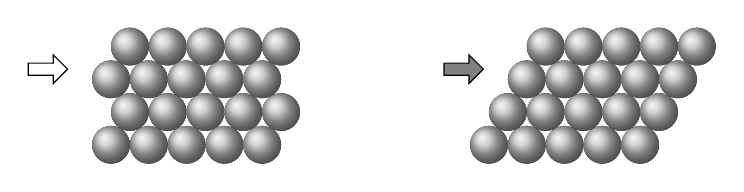
\begin{tikzpicture}[>=stealth,scale=1.2,inner sep=2pt]
  \begin{scope}
  \tkzDefPoint(0,0){A}
  \tkzDefPoint(60:0.4){B}
  \tkzDefShiftPoint[B](120:0.4){C}
  \tkzDefShiftPoint[C](60:0.4){D}
  \foreach \r in {0,1,2,3,4}
    { 
      \foreach \x in {A,B,C,D}
      \fill[ball color=lightgray]([shift=(0:0.4*\r)]\x)circle(0.2);
    }
  \end{scope}
  \begin{scope}[xshift=4cm]
  \foreach \r in {0,1,2,3}
    { 
      \foreach \x in {0,1,2,3,4}
      {\fill[ball color=lightgray]([shift=(60:0.4*\r)]0:0.4*\x)circle(0.2);}
    }
  \end{scope}
  \node at (-0.7,0.8)[single arrow,draw,single arrow head extend=3pt,minimum height=0.5cm]{};
  \node at (3.7,0.8)[single arrow,draw,single arrow head extend=3pt,minimum height=0.5cm,fill=gray]{};
\end{tikzpicture}
\end{document}